% Supplementary Materials --- GBFS Audit Catalogue (Computer Standards & Interfaces)
% Standalone companion to manuscript.tex. Cross-references to the main text are
% resolved via the xr package reading manuscript.aux (build order: compile
% manuscript first, then this file, then manuscript again).
\documentclass[11pt,a4paper]{article}
\usepackage[T1]{fontenc}
\usepackage[utf8]{inputenc}
\usepackage{lmodern}
\usepackage[margin=2.5cm]{geometry}
\usepackage{microtype}
\usepackage{amssymb,amsmath,amstext}
\usepackage{booktabs}
\usepackage{longtable}
\usepackage{graphicx}
\usepackage{adjustbox}
\graphicspath{{figures/}}
\usepackage{xcolor}
\usepackage{url}
\usepackage[colorlinks=true,linkcolor=blue,citecolor=blue,urlcolor=blue]{hyperref}
\usepackage{caption}
\usepackage{xr}
\externaldocument{manuscript}
\begin{document}

\section*{Supplementary Materials}
This appendix collects the granular tables and figures extracted from the main
text to keep the narrative focused on the taxonomy, its empirical impact
and its validation. Each is reproducible from the released parquet and
the audit scripts.

\setcounter{table}{0}\renewcommand{\thetable}{S\arabic{table}}
\setcounter{figure}{0}\renewcommand{\thefigure}{S\arabic{figure}}

\paragraph{S1 --- A4 outlier-detector sensitivity to $\sigma$.}

\begin{table}[!htbp]
\centering
\caption{A4 sensitivity sweep on the released v1.0.1 parquet
(46{,}307 stations, 123 systems). Each row reports the absolute
A4 count and four invariance metrics against the $\sigma = 3$
reference: Kendall's $\tau$ on the rank order of the Top-10 cities
(\textbf{T10c}) and Top-10 operators (\textbf{T10o}) by certified
docked-bike count, plus Jaccard similarity on the Top-10 and
Top-50 sets (\textbf{J10c/J50c, J10o/J50o}). Top-10 city
membership is invariant ($J = 1.000$) across the grid;
$\tau \geq 0.956$ throughout.}
\label{tab:a4-sigma-sweep}
\small
\begin{tabular}{@{}rrrrrrrrrr@{}}
\toprule
\textbf{$\sigma$} & \textbf{A4 st.} & \textbf{A4 sys.} & \textbf{Share}
 & \textbf{$\tau$ T10c} & \textbf{$\tau$ T10o}
 & \textbf{J10c} & \textbf{J50c} & \textbf{J10o} & \textbf{J50o}\\
\midrule
2.0 & 597 & 89 & 1.29\,\% & 0.956 & 0.956 & 1.000 & 1.000 & 1.000 & 1.000 \\
2.5 & 543 & 88 & 1.17\,\% & 0.956 & 0.956 & 1.000 & 1.000 & 1.000 & 1.000 \\
\textbf{3.0} & \textbf{500} & \textbf{88} & \textbf{1.08\,\%} & ref. & ref. & ref. & ref. & ref. & ref. \\
3.5 & 459 & 82 & 0.99\,\% & 1.000 & 1.000 & 1.000 & 0.961 & 1.000 & 1.000 \\
4.0 & 415 & 80 & 0.90\,\% & 1.000 & 0.956 & 1.000 & 0.961 & 1.000 & 1.000 \\
\bottomrule
\end{tabular}

\medskip
{\footnotesize \textbf{Methodological caveat on the MAD scale.}
The robust $3\sigma$ A4 detector uses
$\hat\sigma = 1.4826 \cdot \mathrm{MAD}$ as a Gaussian-consistent
scale estimator. This assumes an approximately unimodal,
isotropic spatial distribution of stations per system. For
systems whose deployment is intrinsically anisotropic (transit
corridors, riverside linear networks) the MAD over-estimates the
effective dispersion on the dominant axis and the detector
\emph{under}-flags peripheral stations on that axis; for
\emph{multi-modal} deployments (nationwide systems clustering
around many city centres; see the \emph{Call a Bike} case in
Table~\ref{tab:e5-pilot}) the single-centroid construction
\emph{over}-flags. The threshold sweep above measures the
sensitivity of the detector to its own $\sigma$ parameter; it
does not measure the sensitivity to the underlying geometric
assumption, which is a known limitation and the subject of the
sub-system-clustering refinement noted in
Section~\ref{secDiscussion}.}
\end{table}

\paragraph{S2 --- Empirical distribution of the A6 zero-capacity rate.}
The zero-capacity rate $r_s^{A6}$ across the 301 docked systems with
at least 20 stations is reported in Table~\ref{tab:a6-distribution};
it underpins the $\tau_{A6} = 1\,\%$ threshold of
Section~\ref{secA6Formalisation}.

\begin{table}[!htbp]
\centering
\caption{Empirical distribution of the zero-capacity rate
$r_s^{A6}$ across the 301 docked systems with at least 20 stations and
a reachable \texttt{station\_information} feed. Free-floating systems,
where $c = 0$ is uninformative, are excluded from the A6 base.}
\label{tab:a6-distribution}
\small
\begin{tabular}{@{}lrr@{}}
\toprule
\textbf{Bucket} & \textbf{Systems} & \textbf{Share}\\
\midrule
$r_s^{A6} = 0$\,\% (no $c = 0$)   & 268 & 89.0\,\% \\
$0 < r_s^{A6} \leq 0.5$\,\%        &   7 &  2.3\,\% \\
$0.5 < r_s^{A6} \leq 1$\,\%        &   4 &  1.3\,\% \\
$1 < r_s^{A6} \leq 2$\,\%          &  10 &  3.3\,\% \\
$2 < r_s^{A6} \leq 5$\,\%          &   8 &  2.7\,\% \\
$5 < r_s^{A6} \leq 10$\,\%         &   2 &  0.7\,\% \\
$r_s^{A6} > 10$\,\%                &   2 &  0.7\,\% \\
\midrule
\textbf{Summary statistics} & & \\
\quad mean $\bar r$                 &  0.36\,\% & \\
\quad standard deviation $\hat\sigma$ &  2.41\,\% & \\
\quad systems with $r_s^{A6} \geq \tau_{A6} = 1\,\%$ & 22 & \\
\bottomrule
\end{tabular}
\end{table}

\paragraph{S3 --- Empirical distribution of the A7 null-capacity rate.}
The NaN-capacity rate $\rho_s^{A7}$ across the 640 globally audited
systems with at least 20 stations is reported in
Table~\ref{tab:a7-distribution}; its sharp bimodality justifies the
coarse $\tau_{A7} = 0.5$ threshold of Section~\ref{secA7Formalisation}.

\begin{table}[!htbp]
\centering
\caption{Empirical distribution of the NaN-capacity rate
$\rho_s^{A7}$ across the 640 globally audited systems with at least
20 stations and a reachable \texttt{station\_information} feed.
The corpus is sharply bimodal at the extreme values, which justifies
a coarse threshold rather than a distribution-anchored one.}
\label{tab:a7-distribution}
\small
\begin{tabular}{@{}lrr@{}}
\toprule
\textbf{Bucket} & \textbf{Systems} & \textbf{Share}\\
\midrule
$\rho_s^{A7} = 0$\,\% (no NaN)        & 238 & 37.2\,\% \\
$0 < \rho_s^{A7} < 1$\,\%              &   4 &  0.6\,\% \\
$1 \leq \rho_s^{A7} < 10$\,\%          &  11 &  1.7\,\% \\
$10 \leq \rho_s^{A7} < 50$\,\%         &  22 &  3.4\,\% \\
$50 \leq \rho_s^{A7} < 99$\,\%         &  41 &  6.4\,\% \\
$99 \leq \rho_s^{A7} < 100$\,\%        &   5 &  0.8\,\% \\
$\rho_s^{A7} = 100$\,\% (all NaN)      & 319 & 49.8\,\% \\
\midrule
\textbf{Mass at the two extremes} & 557 & \textbf{87.0\,\%} \\
\bottomrule
\end{tabular}
\end{table}


\paragraph{Released catalogue schema (column families).}

\begin{table}[!htbp]
\centering
\caption{Column families of \texttt{stations\_gold\_standard\_final.parquet}
(46 typed columns). Columns marked $^\dag$ are produced by the audit
pipeline; $^\ast$ are derived from external sources. The full per-column
schema (name, dtype, source, completeness) ships as a JSON Schema, a
Frictionless Data Package and a Croissant manifest
(\texttt{catalogue/metadata/}). The \texttt{audit\_confidence} enum is
\emph{high} when no flag fires, \emph{medium} for a single A3 or A7 flag,
and \emph{low} otherwise.}
\label{tab:schema}
\small
\begin{tabular}{@{}lrl@{}}
\toprule
\textbf{Family} & \textbf{Cols} & \textbf{Examples / source}\\
\midrule
Identifiers                   & 5  & \texttt{uid}, \texttt{station\_id}, \texttt{system\_id}\\
Spatial \& administrative     & 6  & \texttt{lat}/\texttt{lon}, \texttt{city}, INSEE commune/region\\
Station description           & 4  & name, address, \texttt{capacity}, \texttt{n\_stations\_system}\\
Audit pipeline outputs$^\dag$ & 13 & \texttt{station\_type}, \texttt{capacity\_raw}/\texttt{\_audited}, \texttt{flag\_A1}--\texttt{A7}, \texttt{audit\_confidence}\\
Network geometry$^\dag$       & 5  & intra-/inter-system KNN distances, local densities\\
Topography$^\ast$             & 2  & elevation, roughness (IGN BD ALTI)\\
Cycling infrastructure$^\ast$ & 2  & cycle-lane linear \& share (IGN BD TOPO)\\
Safety$^\ast$                 & 1  & severe cyclist crashes (ONISR BAAC)\\
Multimodal access$^\ast$      & 2  & heavy-transit stops within 300\,m (GTFS)\\
Socio-economic context$^\ast$ & 5  & INSEE Filosofi income, Gini, car-less share\\
Modal share$^\ast$            & 1  & commute-by-bike share (INSEE)\\
\midrule
\textbf{Total}                & \textbf{46} & \\
\bottomrule
\end{tabular}
\end{table}

\paragraph{Reference sources for contextual enrichment.}

\begin{table}[!htbp]
\centering
\caption{Reference sources used for contextual enrichment. Every
listed source contributes at least one column to the released
parquet schema (Table~\ref{tab:schema}). Out-of-scope sources
considered during prototyping but not retained in the v1.0
release (OpenStreetMap point-of-interest density, FUB cycling
barometer score) are documented in the audit report.}
\label{tab:sources}
\small
\begin{tabular}{@{}llll@{}}
\toprule
\textbf{Source} & \textbf{Granularity} & \textbf{Variables} &
\textbf{Operation}\\
\midrule
INSEE Filosofi      & IRIS / municipality &
   Median income/CU, local Gini, decile, car-less share & Aggregation \\
INSEE Recensement   & municipality &
   Share of commute by bike (\texttt{part\_velo\_travail})  & Aggregation \\
IGN BD ALTI         & DEM raster &
   Elevation, topographic roughness index & Spatial sampling \\
IGN BD TOPO         & polylines &
   Cycle-infrastructure linear (300\,m buffer) & Spatial join \\
ONISR BAAC (Cerema) & geolocated accident &
   Severe-crash count (500\,m, 5\,yr) & Spatial join \\
National GTFS aggregator & GTFS stops &
   Heavy-transit stops within 300\,m & Spatial join \\
\bottomrule
\end{tabular}
\end{table}

\paragraph{Per-country breakdown of structural classes A1--A4.}

\begin{table}[!htbp]
\centering
\caption{Per-country breakdown of the four structural classes
A1--A4 on the MobilityData canonical catalogue (1{,}509 systems,
including the 255 French entries). The macro-region class A5
(17 systems globally), zero-capacity A6 (22) and null-capacity A7
(245 / 97{,}314 stations) are calibrated on station-count-conditioned
sub-corpora and are reported in
Tables~\ref{tab:a6-distribution} and \ref{tab:a7-distribution}.
Per-class counts are not disjoint; ``Flagged'' aggregates A1--A5
only. Countries with $\geq 30$ audited systems or notable hotspot
concentrations are shown. A4 requires both $>5\,\%$ of stations
and $\geq 5$ absolute outside-country stations to flag, to avoid
edge-of-coast false positives.}
\label{tab:global-audit}
\small
\begin{tabular}{@{}lrrrrrrr@{}}
\toprule
\textbf{Country} & \textbf{Audited} & \textbf{Reach.} & \textbf{Flagged}
   & \textbf{A1} & \textbf{A2} & \textbf{A3} & \textbf{A4 geo}\\
\midrule
\textbf{France (FR)}      & 255 & 253 & \textbf{38} & 17 & 14 &  4 &  3 \\
Germany (DE)              & 251 & 243 & 32 & 21 &  4 &  9 & -- \\
United States (US)        & 175 & 172 &  0 & -- & -- & -- & -- \\
Poland (PL)               &  94 &  91 & 28 & -- &  3 & -- & 25 \\
Norway (NO)               &  83 &  46 &  2 & -- & -- & -- &  2 \\
Spain (ES)                &  69 &  66 &  1 & -- & -- & -- &  1 \\
United Kingdom (GB)       &  56 &  54 &  3 & -- &  1 & -- &  2 \\
Finland (FI)              &  55 &  55 & 14 & -- & -- & -- & 14 \\
Netherlands (NL)          &  52 &  52 &  1 & -- & -- & -- &  1 \\
Switzerland (CH)          &  49 &  46 & 15 &  8 &  3 &  3 &  1 \\
\textbf{Czech Rep.\ (CZ)} &  45 &  43 & \textbf{25} & -- & \textbf{16} & \textbf{12} & -- \\
Belgium (BE)              &  37 &  34 &  4 & -- & -- &  2 &  2 \\
Italy (IT)                &  34 &  33 &  0 & -- & -- & -- & -- \\
Austria (AT)              &  27 &  23 &  1 & -- &  1 &  1 & -- \\
Sweden (SE)               &  23 &  23 & 12 & -- & -- & -- & 12 \\
Slovakia (SK)             &  19 &  19 & 16 & -- & -- & -- & 16 \\
\midrule
\textbf{Total (48 countries)} & 1{,}509 & 1{,}420 & 204 & 46 & 48 & 33 & 81 \\
\bottomrule
\end{tabular}

\medskip
{\footnotesize \emph{Reproducibility.}~Per-country counts produced by
\texttt{scripts/audit\_live\_systems.py -{}-infer-type} against the
1{,}509-system MobilityData catalogue; the \texttt{-{}-infer-type}
flag activates operator-name heuristics (regexes for car-sharing /
free-floating brands listed at the top of the script) required to
fire A1 and A3 where \texttt{station\_type} is not declared.
Numbers re-fetched later will drift as feeds evolve; the 2026-04 snapshot
used here is archived under
\texttt{experiments/e2\_threshold\_sensitivity/global\_audit\_snapshot/}
(run \texttt{verify\_snapshot.py} to reproduce these counts). The sibling
\texttt{global\_audit\_results\_typed.csv} is a later 2026-05 re-crawl and
does not match these figures.}
\end{table}

\paragraph{Urban areas most affected by the purging protocol.}

\begin{table}[!htbp]
\centering
\caption{Top five French urban areas most affected by the purging
protocol. ``Raw'' is the count of \texttt{station\_information}
entries in the unaudited feed; ``Cert.\ dock'' is the count of
dock-based stations in the Audit Catalogue. The drop is essentially
the share of GBFS entries that the audit reclassifies as
free-floating (A3), car-sharing (A1), or filtered (A4--A5). The
``Flags driving the drop'' column lists the anomaly classes that
each agglomeration's flagged systems trigger.}
\label{tab:top5-reranks}
\small
\begin{tabular}{@{}lrrrl@{}}
\toprule
\textbf{Urban area} & \textbf{Raw} & \textbf{Cert.\ dock}
                    & \textbf{Drop} & \textbf{Flags driving the drop}\\
\midrule
Bordeaux         & 9{,}921 & 225   & $-97.7\,\%$
                 & A3 (Pony), A1 (Citiz), A7 (Dott, Bird) \\
Paris            & 19{,}872 & 1{,}507 & $-92.4\,\%$
                 & A7 (Dott, Bird), A3 (Pony Paris) \\
Marseille        & 2{,}391 & 221   & $-90.8\,\%$
                 & A3 (Pony), A7 (Dott) \\
Strasbourg       & 310     & 39    & $-87.4\,\%$
                 & A1 (Citiz Grand Est) \\
Lyon             & 2{,}057 & 452   & $-78.0\,\%$
                 & A3 (Pony, Bird), A7 (Dott) \\
\bottomrule
\end{tabular}
\end{table}

\paragraph{Empirical distribution of the A3 capacity-profile ratio.}

\begin{table}[!htbp]
\centering
\caption{Empirical distribution of
$\bar c_{\text{profile}}/\bar c_{\text{actual}}$ across two
corpora: the 95 audited French systems with non-empty
\texttt{capacity} (split docked / free-floating; the derivation
set) and the 267 globally audited systems (live sweep across 33
countries, station\_type unknown for many; the out-of-sample
set). The threshold $\tau_{A3} = 5$ is preserved in this paper
as a conservative cut-off; the global distribution shows that
the band $[2, 5]$ is not empty (15 systems) and that a future
revision of A3 may benefit from a soft / hard two-tier
threshold analogous to A6.}
\label{tab:a3-threshold-empirical}
\small
\begin{tabular}{@{}lrrr@{}}
\toprule
& \multicolumn{2}{c}{\textbf{French corpus (n = 95)}} & \textbf{Global (n = 267)}\\
\cmidrule(lr){2-3} \cmidrule(lr){4-4}
\textbf{Ratio bucket} & \textbf{Docked} & \textbf{Free-floating} & \textbf{All}\\
\midrule
$[1.00, 1.10]$    & 79 & 9$^\dag$ & 197 \\
$[1.10, 2.00]$    & 2  & 0        & 24 \\
$[2.00, 5.00]$    & 0  & 0        & 15 \\
$[5.00, 20.00]$   & 0  & 0        & 12 \\
$[20.00, 50.00]$  & 0  & 0        & 9 \\
$[50.00, \infty)$ & 0  & 5        & 10 \\
\midrule
\textbf{Total}    & 81 & 14       & 267 \\
\bottomrule
\end{tabular}

\medskip
{\footnotesize $^\dag$ Two qualitatively different cases populate
the lowest bucket. The 79 docked French systems carry stable
positive capacities so $\bar c_{\text{profile}}$ and
$\bar c_{\text{actual}}$ coincide by virtue of \emph{the data};
the 9 free-floating French systems sit there by virtue of
\emph{the arithmetic}, because their capacity column is mostly
NaN or zero and the ratio degenerates to unity rather than
reflecting the conditional-averaging publication choice. The
same indistinguishability affects the global ``All'' column,
where we cannot a-priori separate clean docks from degenerate-FF
without a per-system audit; the top 10 global systems by ratio
are however all known free-floating operators (Pony, nextbike,
Voi, Bolt), so the $[5, \infty)$ tail tracks the A3 mechanism
across the sweep.}
\end{table}

\paragraph{A4 ablation: legacy versus topology-aware detector.}

\begin{figure}[!htbp]
\centering

\includegraphics[width=0.95\linewidth]{fig09_xp2_ablation_overview.pdf}
\caption{Ablation of the centroid-based A4 detector against the
topology-aware composite detector. \emph{Left}: discordance
classification across all 46{,}307 stations. \emph{Centre}:
legacy false positives stratified by system geometry type (isotropic
vs.\ linear). \emph{Right}: scatter of legacy $\sigma$-distance
against composite anomaly score, coloured by discordance class;
dashed lines mark the respective detection thresholds.}
\label{fig:ablation}
\end{figure}

\paragraph{Leave-one-operator-out cross-validation overview.}

\begin{figure}[!htbp]
\centering

\includegraphics[width=0.95\linewidth]{fig10_xp3_looo_overview.pdf}
\caption{LOOO cross-validation overview. \emph{Top-left}: per-rule
coefficient of variation (green = CV $< 0.20$, red = above).
\emph{Top-right}: mean flag rate with 95\,\% bootstrap CI.
\emph{Bottom-left}: heatmap of per-operator flag rates on the
test fold. \emph{Bottom-right}: test/train flag-rate ratio
(ratio $\approx 1$ indicates operator-agnostic behaviour).}
\label{fig:looo}
\end{figure}

\paragraph{Mapping of the purging protocol to ISO/IEC 25012.}

\begin{table}[!htbp]
\centering
\caption{Mapping of the nine-step purging-protocol design properties
to the data-quality dimensions of ISO/IEC~25012:2008 and its
companion measurement standard ISO/IEC~25024:2015. The Audit
Catalogue is, to our knowledge, the first FAIR-released
implementation of these dimensions on a GBFS corpus.}
\label{tab:iso-mapping}
\small
\begin{tabular}{@{}lll@{}}
\toprule
\textbf{Protocol property}     & \textbf{ISO/IEC~25012 dimension}   & \textbf{Mechanism in the pipeline}\\
\midrule
Idempotence                    & Internal consistency               & Unit-tested re-application on certified output\\
Reversibility                  & Recoverability + Traceability      & \texttt{rejected\_stations.parquet} with exclusion motive\\
Step-level logging             & Traceability                       & Per-step in/out counts and transformation type\\
Explicit parameterisation      & Understandability                  & Hyperparameters in code + documented in audit report\\
FAIR release                   & Compliance + Accessibility         & JSON Schema, DCAT-AP, Croissant, ODbL on Zenodo\\
Blind author cross-annotation  & Accuracy + Semantic consistency    & Author-led consistency check that flagged anomalies are real defects (Section~\ref{secHumanVal})\\
\bottomrule
\end{tabular}
\end{table}



\paragraph{Urban areas most affected by the A3 reclassification.}

\begin{figure}[!htbp]
\centering
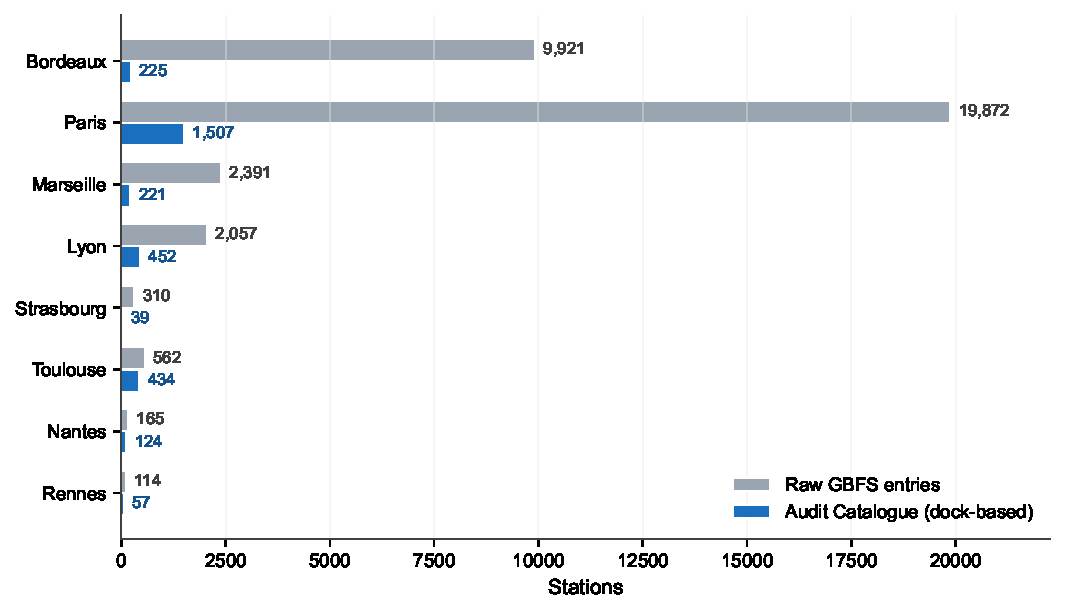
\includegraphics[width=0.9\linewidth]{fig04_bordeaux_before_after.pdf}
\caption{Top twelve French urban areas ranked by absolute reduction in
dock-based station count between the raw GBFS feed and the certified
Audit Catalogue. \textbf{Bordeaux} (highlighted) exhibits the largest
absolute drop, driven by the reclassification of the \emph{Pony}
free-floating fleet (A3). Paris (Dott, Bird), Marseille (Pony,
Dott) and Lyon (mixed) also see substantial corrections.}
\label{fig:bordeaux-before-after}
\end{figure}

\paragraph{Completeness of contextual enrichment.}

\begin{figure}[!htbp]
\centering
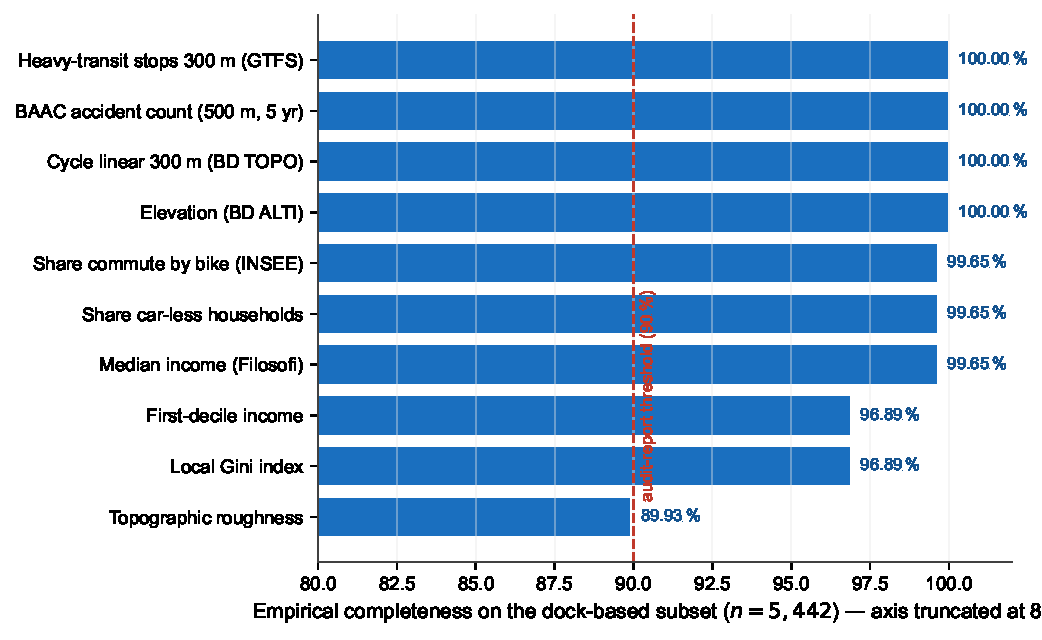
\includegraphics[width=0.7\linewidth]{fig05_completeness.pdf}
\caption{Empirical completeness of contextual enrichment per
derived variable on the dock-based subset of the Audit Catalogue
($n = 5{,}442$). All variables exceed the $90\,\%$ completeness
threshold required by the audit report; missing values remain below
$6\,\%$ across the corpus.}
\label{fig:completeness}
\end{figure}

\paragraph{Per-country incidence of structural classes A1--A4.}

\begin{figure}[!htbp]
\centering
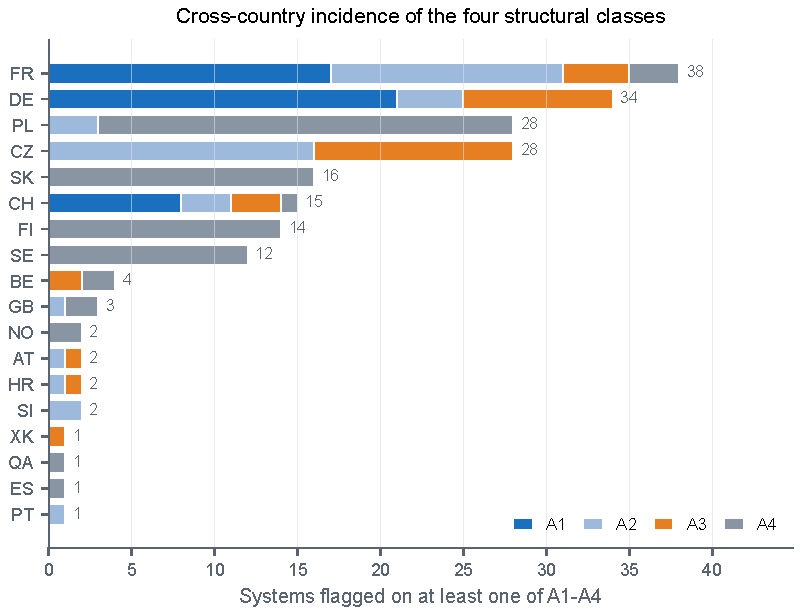
\includegraphics[width=0.92\linewidth]{fig07_global_audit.pdf}
\caption{Per-country incidence of the structural classes A1--A4 across
the 1{,}509-system MobilityData catalogue (top 18 countries by total
flagged). The chart shows the stacked composition of the
\textbf{Flagged} column of Table~\ref{tab:global-audit} and makes the
country-level signatures legible at a glance: A4 (geospatial) drives
the Polish, Finnish, Swedish and Slovak hotspots (cross-border bounding
boxes on aggregator feeds), A1 (car-sharing labelled as BSS) drives
the DACH cluster (Germany, Switzerland), A2 (placeholder capacity) and
A3 (over-capacity) drive France and the Czech Republic. Macro-region
(A5), zero-capacity (A6) and null-capacity (A7) are reported separately
because they are calibrated on station-count-conditioned sub-corpora
(Tables~\ref{tab:a6-distribution} and~\ref{tab:a7-distribution}).}
\label{fig:global-audit-overview}
\end{figure}

\paragraph{Nine falsifiable experiments mapped to the limitations.}

\begin{table}[!htbp]
\centering
\caption{Nine falsifiable experiments mapped to the limitations of
Section~\ref{secLimitations}. ``$\checkmark$'' = completed result
reported in this paper; ``Pilot $\checkmark$'' = preliminary result
already reported; full protocols and reproduction scripts ship under
\texttt{experiments/} in the source repository.}
\label{tab:roadmap}
\small
\begin{tabular}{@{}llll@{}}
\toprule
\textbf{ID} & \textbf{Title} & \textbf{Targets} & \textbf{Status}\\
\midrule
E1 & Pre-registered held-out audit (post-freeze MobilityData) & Construct validity / circularity & Retrospective version executed (2/3 H pass) $\checkmark$ \\
E2 & Threshold and buffer sensitivity           & $\sigma_{\max}, N_{\min}$, radii & $\sigma_{\max}$ pilot $\checkmark$ \\
E3 & Twelve-month temporal stability            & Snapshot dependence (L4)    & Running \\
E4 & Dynamic extension to \texttt{station\_status} & L2                       & 2-day pilot $\checkmark$; Shannon protocol ready \\
E5 & European generalisation (live audit, 6 tech stacks) & L1                  & 13-system panel $\checkmark$ \\
E6 & Free-floating-native protocol              & L3                          & Planned 2027-Q2 \\
\textbf{E7} & \textbf{A4\,v2 topology-aware ablation} & \textbf{Geospatial isotropy bias} & \textbf{$\checkmark$ (Sec.~\ref{secA4v2})} \\
\textbf{E8} & \textbf{Leave-one-operator-out CV}       & \textbf{Overfitting (H3)}          & \textbf{$\checkmark$ (Sec.~\ref{secLOOO})} \\
\textbf{E9} & \textbf{Dynamic station\_status audit} & \textbf{Static/dynamic gap (L2)}  & \textbf{Future work (pipeline shipped)} \\
\bottomrule
\end{tabular}
\end{table}

\end{document}
